\section{Experiments}
\label{sec:experiments}

The experiments are organized around the belief-update mechanism rather than around user interaction alone. We first evaluate how the confidence threshold $\tau$ affects task success, execution length, and query frequency. This analysis directly tests the role of entropy-normalized confidence in deciding when belief can be committed to the knowledge base. We then compare query policies to isolate the value of belief-triggered, hypothesis-level querying. A compact user study is included as a secondary analysis of the human-facing consequences of these policies.

\subsection{Domains}
\label{sec:domains}

\begin{figure}[t]
    \centering
    \begin{subfigure}[b]{0.47\linewidth}
        \centering
        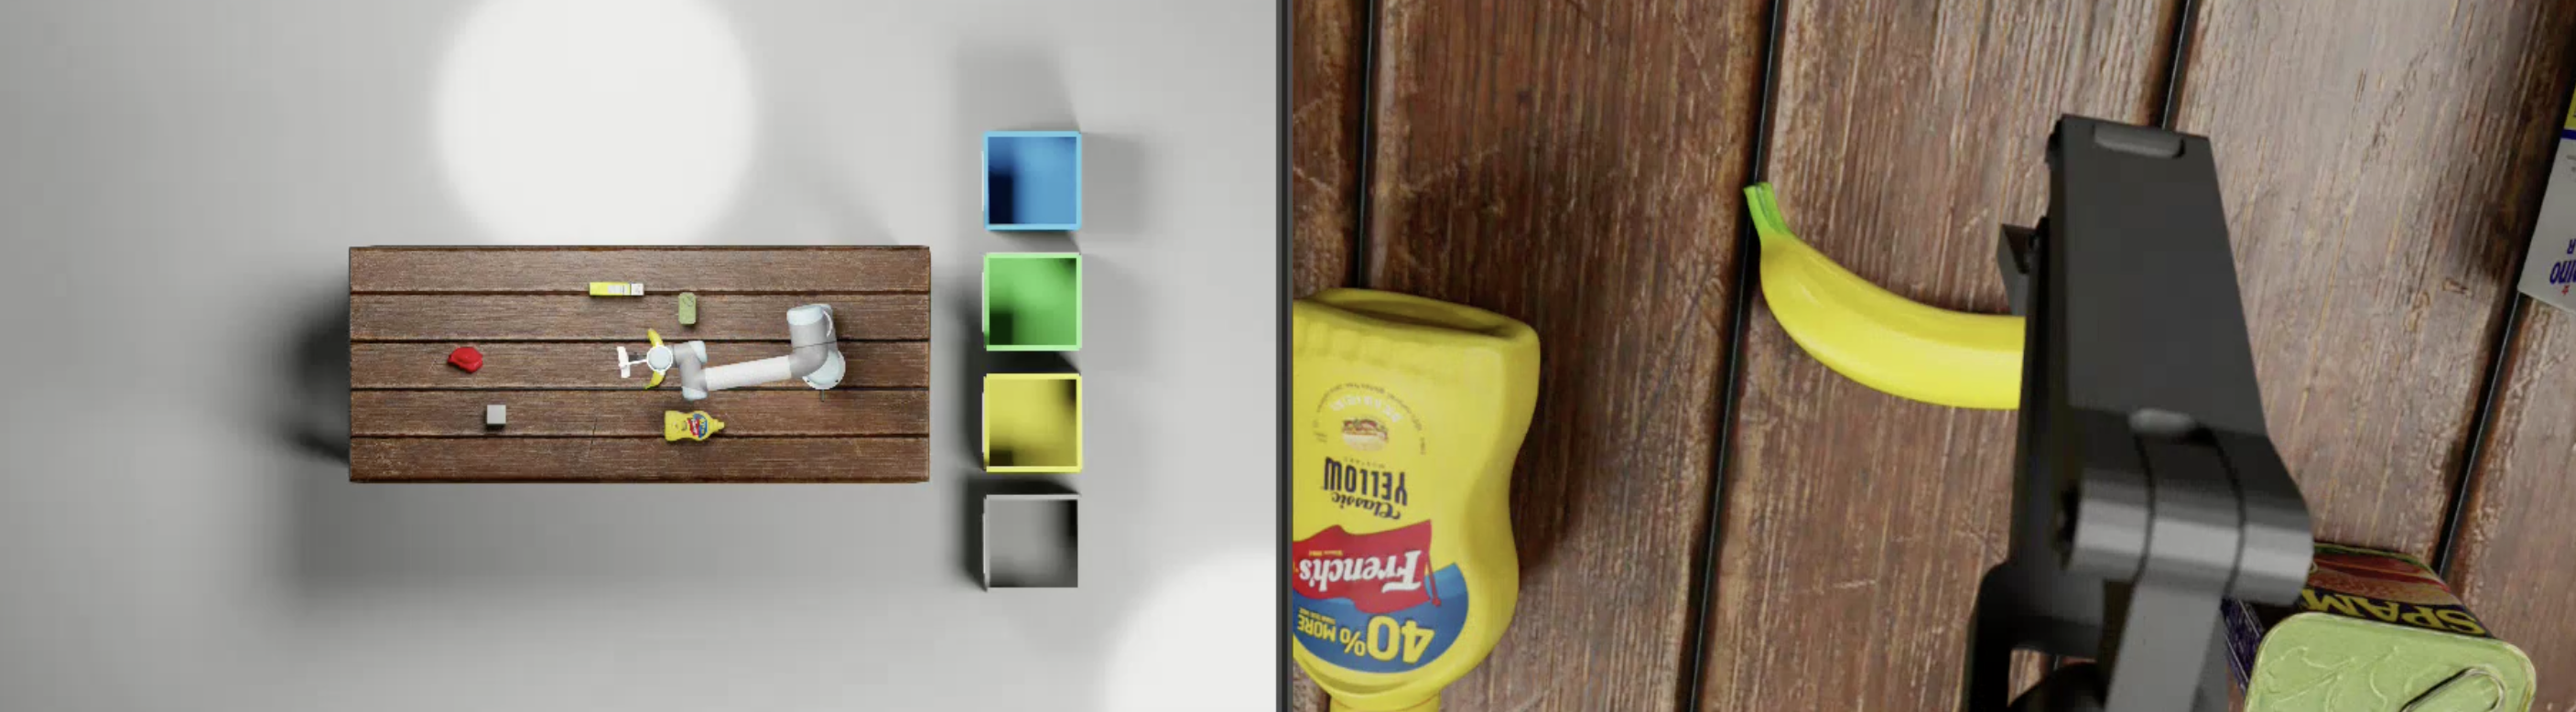
\includegraphics[width=\linewidth]{figures/fig_exp_setup1.png}
        \caption{Waste sorting.}
        \label{fig:domain_waste}
    \end{subfigure}
    \hfill
    \begin{subfigure}[b]{0.47\linewidth}
        \centering
        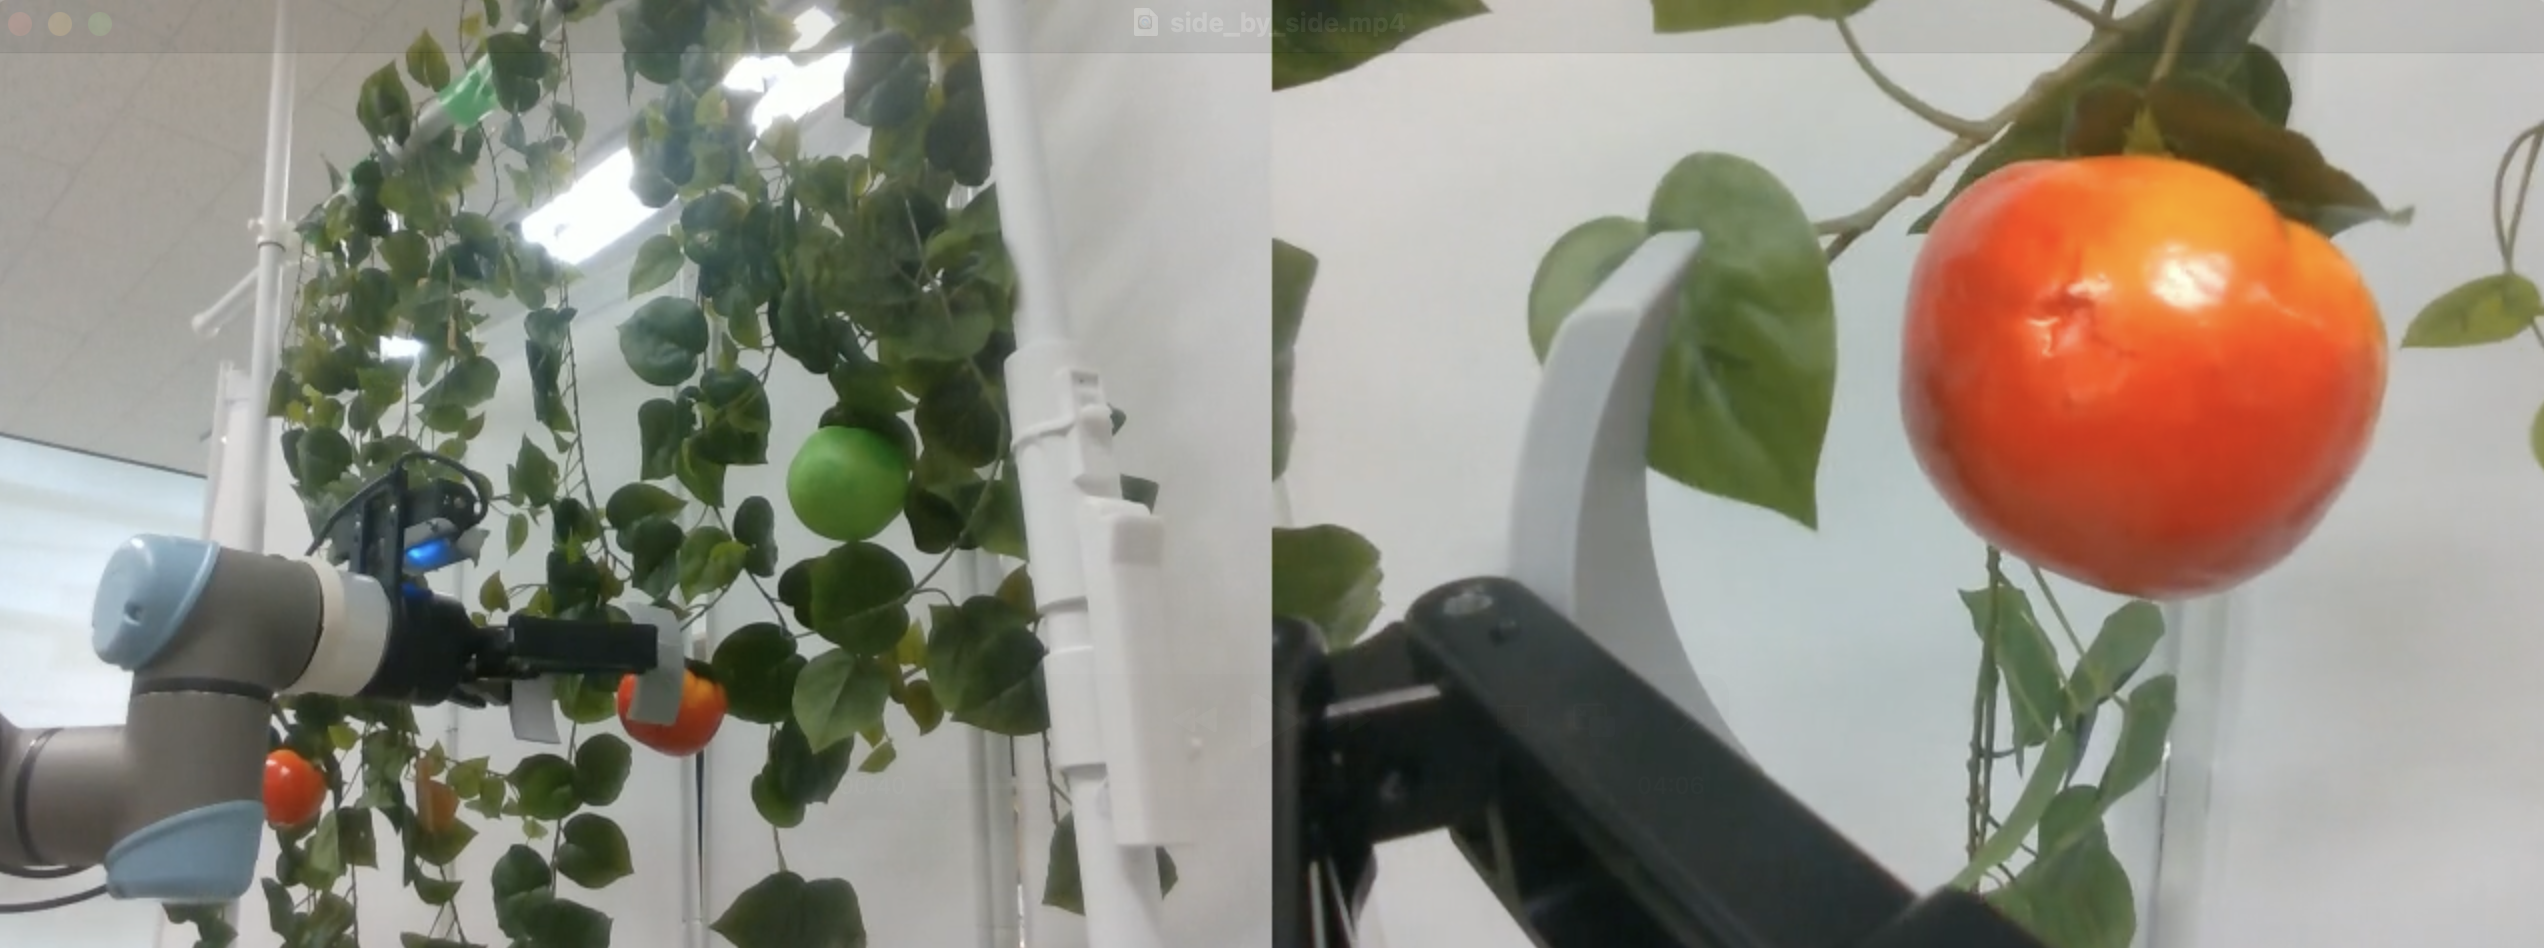
\includegraphics[width=\linewidth]{figures/fig_exp_setup2.png}
        \caption{Tomato harvesting.}
        \label{fig:domain_tomato}
    \end{subfigure}
    \caption{Experimental domains. The waste sorting domain evaluates symbolic category uncertainty in simulation, while the tomato harvesting domain evaluates uncertainty over tomato states in a robot harvesting task.}
    \label{fig:domains}
\end{figure}

\paragraph{Waste sorting.}
The waste sorting domain consists of a UR5 robot sorting objects into category-specific bins. Each object belongs to one of four categories: general waste, paper, can, or plastic. Categories are not fully known in advance and may be ambiguous due to occlusion or perception uncertainty. The robot must detect, pick, and place objects into the correct bins.

\paragraph{Tomato harvesting.}
The tomato harvesting domain contains tomatoes attached to stems. Each tomato may be ripe, unripe, or rotten. Ripe tomatoes should be harvested, rotten tomatoes should be discarded, and unripe tomatoes should be left untouched. This domain is more sensitive to unresolved local information because a wrong belief about a tomato state can directly cause a wrong harvest or discard.

\subsection{Metrics and Policies}
\label{sec:metrics_policies}

We report task success rate, average number of queries, and average number of execution steps. Query count measures interaction cost, while execution steps measure the downstream planning cost of unresolved belief ambiguity. In the policy comparison, \textbf{All} queries whenever feedback can be generated, \textbf{No} never queries, \textbf{Random} queries without using belief confidence, and \textbf{Ours} queries only when $\mathrm{Conf}(\mathcal{B})<\tau$ and selects the hypothesis minimizing expected posterior entropy.

\subsection{Confidence Threshold Analysis}
\label{sec:threshold_analysis}

\begin{figure}[t]
    \centering
    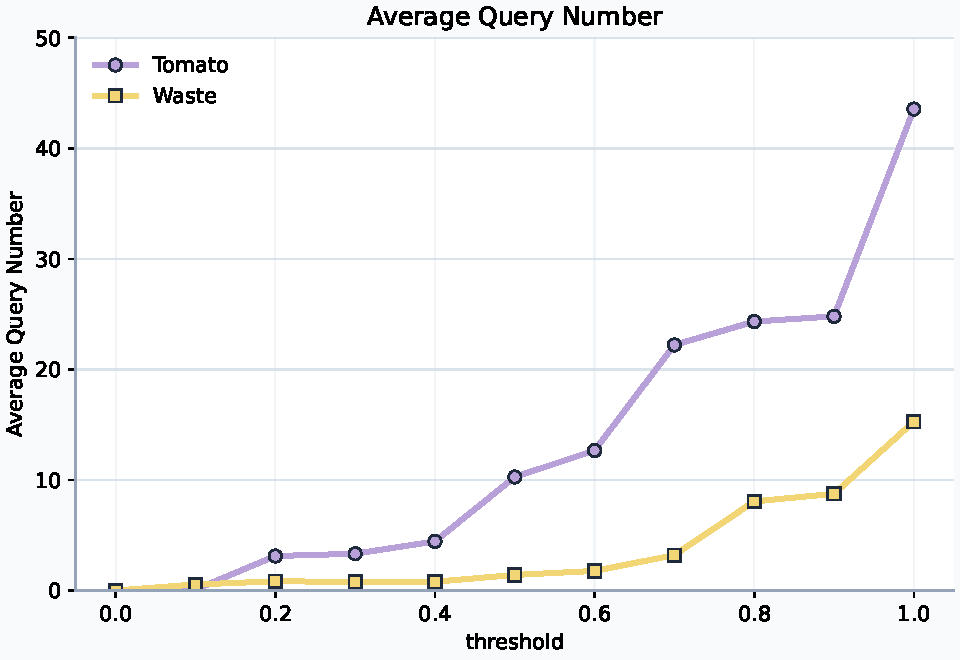
\includegraphics[width=0.31\linewidth]{figures/fig_average_question.pdf}
    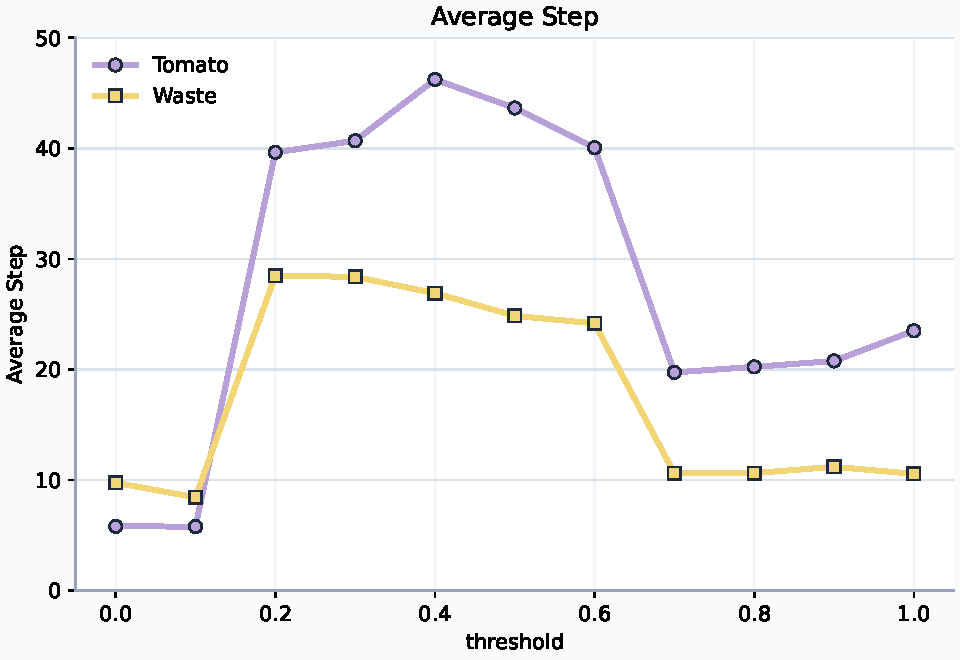
\includegraphics[width=0.31\linewidth]{figures/fig_average_step.pdf}
    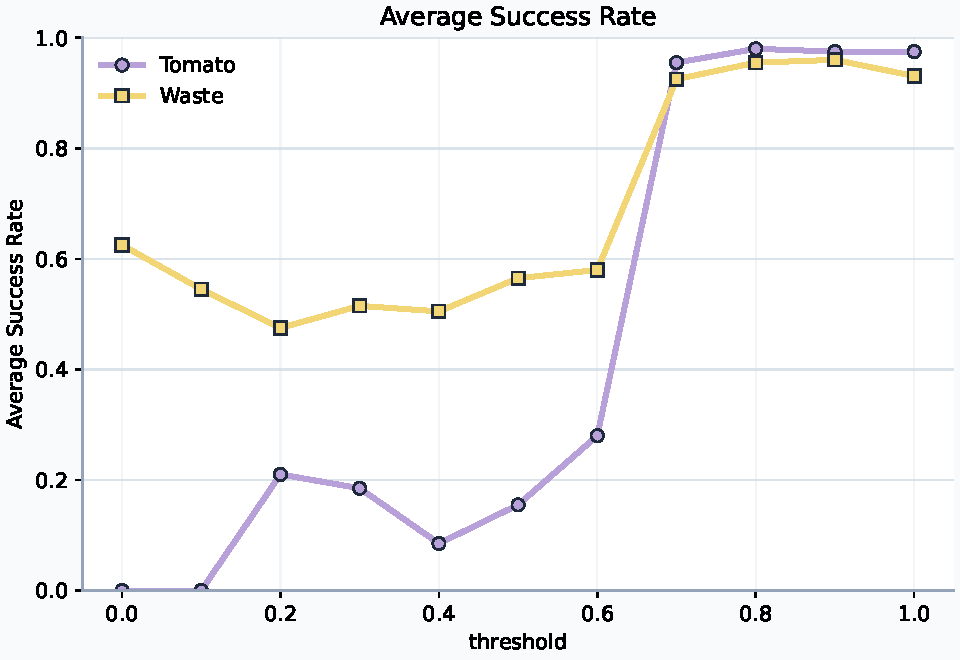
\includegraphics[width=0.31\linewidth]{figures/fig_average_success_rate.pdf}
    \caption{System performance under different confidence thresholds $\tau$. Increasing $\tau$ makes the belief-to-knowledge transition more conservative, increasing query frequency while reducing failures caused by premature commitment.}
    \label{fig:tau_analysis}
\end{figure}

\begin{table}[t]
\centering
\caption{System evaluation under different confidence thresholds $\tau$. Success rates are percentages.}
\label{tab:tau_analysis}
\small
\setlength{\tabcolsep}{3pt}
\begin{tabular}{lcccccc}
\toprule
\multirow{2}{*}{$\tau$} & \multicolumn{3}{c}{\textbf{Waste}} & \multicolumn{3}{c}{\textbf{Tomato}} \\
\cmidrule(lr){2-4}\cmidrule(lr){5-7}
& Success & Queries & Steps & Success & Queries & Steps \\
\midrule
0.0 & 62.5 & 0.0  & 9.7  & 0.0  & 0.0  & 5.8  \\
0.3 & 51.5 & 0.8  & 28.4 & 18.5 & 3.3  & 40.7 \\
0.6 & 58.0 & 1.8  & 24.2 & 28.0 & 12.7 & 40.1 \\
0.7 & 92.5 & 3.2  & 10.6 & 95.5 & 22.2 & 19.7 \\
0.8 & 95.5 & 8.1  & 10.6 & 98.0 & 24.3 & 20.2 \\
0.9 & 96.0 & 8.8  & 11.2 & 97.5 & 24.8 & 20.8 \\
1.0 & 93.1 & 15.3 & 10.6 & 97.5 & 43.5 & 23.5 \\
\bottomrule
\end{tabular}
\end{table}

The threshold analysis shows that $\tau$ acts as a system-level guard on knowledge-base commitment. Low thresholds allow the robot to commit states despite high entropy, which reduces queries but often leaves task-relevant ambiguity unresolved. In tomato harvesting, success remains below $30\%$ through $\tau=0.6$ because the robot frequently commits incorrect local information about tomato states. Increasing $\tau$ from $0.6$ to $0.7$ raises success from $28.0\%$ to $95.5\%$ in tomato harvesting and from $58.0\%$ to $92.5\%$ in waste sorting. This sharp transition indicates that belief confidence is not merely a descriptive statistic; it directly controls whether the symbolic planner acts from stable knowledge or from ambiguous local information.

For $\tau\geq0.7$, both domains maintain success above $92\%$. We use $\tau=0.8$ for policy comparisons because it gives high success in both domains while avoiding the excessive query cost observed at $\tau=1.0$, especially in tomato harvesting.

\subsection{Query Policy Comparison}
\label{sec:policy_comparison}

\begin{figure}[t]
    \centering
    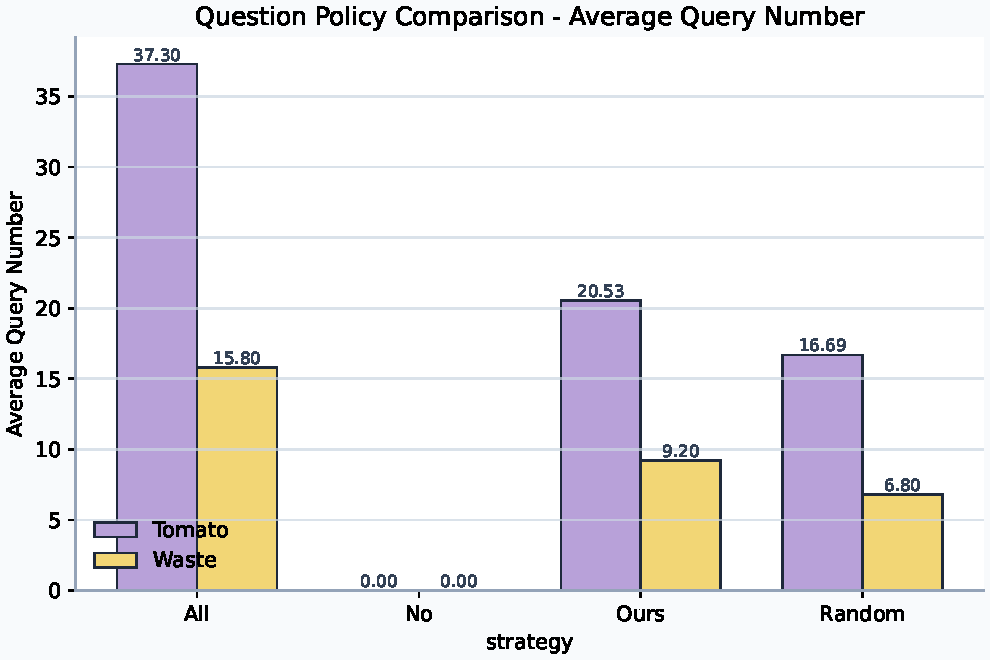
\includegraphics[width=0.31\linewidth]{figures/fig_when_strategy_average_question_domain_compare.pdf}
    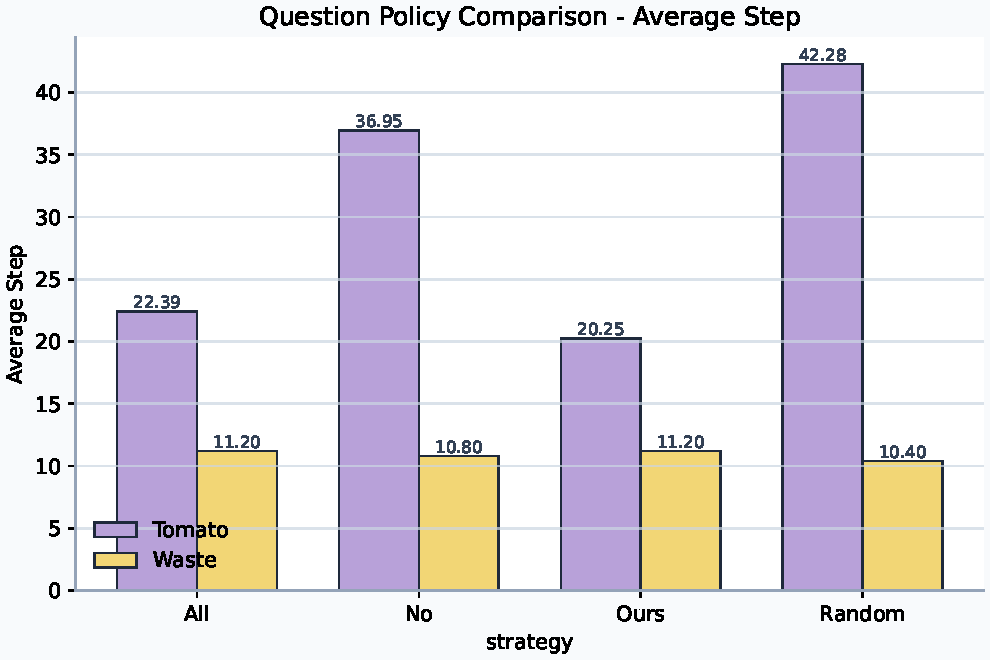
\includegraphics[width=0.31\linewidth]{figures/fig_when_strategy_average_step.pdf}
    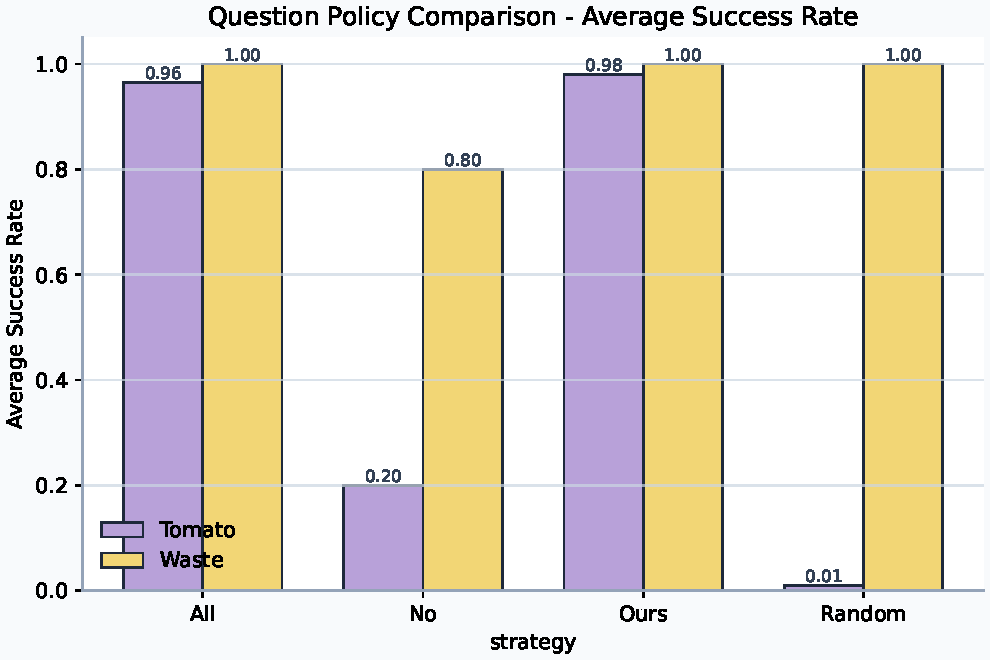
\includegraphics[width=0.31\linewidth]{figures/fig_when_strategy_average_success_rate.pdf}
    \caption{System performance under different query policies at $\tau=0.8$. Belief-triggered querying preserves high success while avoiding the interaction cost of always querying.}
    \label{fig:policy_comparison}
\end{figure}

\begin{table}[t]
\centering
\caption{Query policy comparison at $\tau=0.8$.}
\label{tab:policy_comparison}
\small
\setlength{\tabcolsep}{4pt}
\begin{tabular}{lcccccc}
\toprule
\multirow{2}{*}{\textbf{Policy}} & \multicolumn{3}{c}{\textbf{Waste}} & \multicolumn{3}{c}{\textbf{Tomato}} \\
\cmidrule(lr){2-4}\cmidrule(lr){5-7}
& Success & Queries & Steps & Success & Queries & Steps \\
\midrule
\textbf{All}    & 100.0 & 15.8 & 11.2 & 96.5 & 37.3 & 22.4 \\
\textbf{No}     & 80.0  & 0.0  & 10.8 & 20.0 & 0.0  & 36.9 \\
\textbf{Random} & 100.0 & 6.8  & 10.4 & 1.0  & 16.7 & 42.3 \\
\textbf{Ours}   & 100.0 & 9.2  & 11.2 & 98.0 & 20.5 & 20.2 \\
\bottomrule
\end{tabular}
\end{table}

The policy comparison separates the effect of feedback quantity from the effect of belief-aware timing. In waste sorting, \textbf{All}, \textbf{Random}, and \textbf{Ours} all reach $100.0\%$ success, but \textbf{Ours} reduces queries relative to \textbf{All}. In tomato harvesting, where local state ambiguity is more consequential, \textbf{Ours} reaches $98.0\%$ success with $20.5$ queries on average, while \textbf{All} reaches $96.5\%$ success with $37.3$ queries. \textbf{No} fails frequently because incorrect beliefs are committed without correction, and \textbf{Random} performs poorly because queries are not aligned with the belief states that matter for future planning.

These results support the central system claim: the benefit comes from coupling the query trigger and query content to the frontier belief. Asking more often is not sufficient, and asking less often is not safe unless the system can determine when uncertainty matters for planning.

\subsection{User Study as Secondary Evaluation}
\label{sec:user_study}

The user study is included to check whether the system-level query policy creates reasonable interaction demands for human users. Twelve participants completed waste sorting and tomato harvesting scenarios under five interaction conditions: \textbf{All}, \textbf{No}, \textbf{Ours1}, \textbf{Ours2}, and \textbf{KnowNo}. Because the IJRR framing focuses on the belief-space system, we summarize only the main interaction findings here.

Across both domains, SAGAT-based answer accuracy did not show a significant overall condition effect, but waste sorting showed a significant condition effect: \textbf{Ours1} achieved the highest accuracy ($M=0.72$, $SD=0.15$) and exceeded \textbf{All} ($M=0.56$, $SD=0.19$). The strongest item-level signal came from the question asking why the robot requested information; in waste sorting, \textbf{Ours1} reached perfect accuracy on this item. For workload, \textbf{Ours2} reduced NASA-TLX workload relative to the action-level \textbf{KnowNo} baseline and showed lower effort than both \textbf{All} and \textbf{KnowNo}. These results are consistent with the system view that state-level queries can expose the robot's uncertainty without asking users to take over action selection.
